\section{Experimental Results}

This section reports results for experiments aimed at
answering the three research questions described in Section~\ref{sec:exp}. 

\subsection{National Chokepoint Potential (NCP)} 

We report results for eight countries, some that are known to practice censorship and some that are considered more open.
We selected four well-known countries with
extensive Internet censorship policies: China, Turkey,
Egypt, and Russia. China has historically been the most aggressive in terms of
Internet censorship \cite{censorshipSurvey}. Turkey recently
began blocking social media
accesses during turmoil and pressuring ISPs to block access to certain material~\cite{turkeyCensor}. Egypt's Internet suffered
severe shutdowns during the Arab Spring \cite{arabspring}.
Russian has passed surveillance laws requiring ISPs to provide access to user statistics \cite{censorshipGeography}. 
We also selected Germany, the United States, France, and the
United Kingdom because Internet access for these nations is
considered to be open even though they each have conducted limited Internet
censorship \cite{censorshipSurvey}, 
	
\figurename~\ref{fig:nationsCompare} shows national chokepoint
potential for 2018 for different values of $f$ (x-axis). The
y-axis reports the inverse of the number of ASes required to control fraction $f$ of
paths. We report only in-to-out results
because the results for out-to-in are very similar
for all experiments.  \figurename~\ref{fig:nationsCompare} shows the diverse nature of national topologies. China is one
extreme, where over 80\% of paths can be controlled by a single AS,
%as indicated
%by a NCP of 1.0.
Other nations exhibiting strong chokepoints are Egypt, Turkey, and the United Kingdom. The
nations of the US, France, Germany, and Russia show considerably lower NCP for 2018.  These results are as expected, except for Russia. As an early adopter of the Internet, we speculate that Russia's AS topology evolved before stringent regulations were adopted and this early history dominates our measurements.  



\begin{figure}[ht]
	\centering
	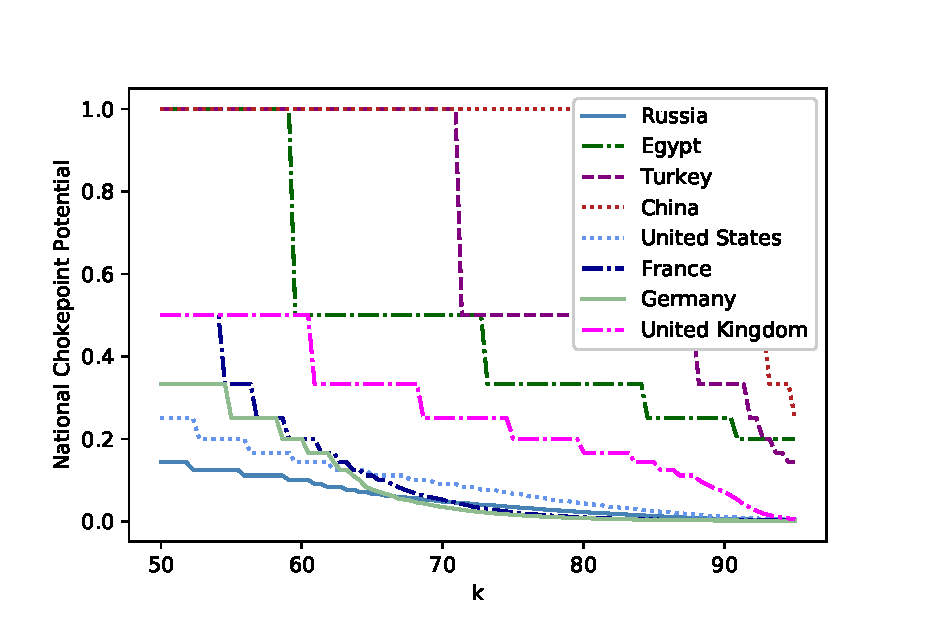
\includegraphics[width=\linewidth]{nationsCompare}
	\caption{The national chokepoint potentials of various nations in 2018. f is the
	fraction of paths used to calculate the national chokepoint potential.}\label{fig:nationsCompare}
\end{figure}

\subsection{Topology Over Time}

\begin{figure}
	\centering
	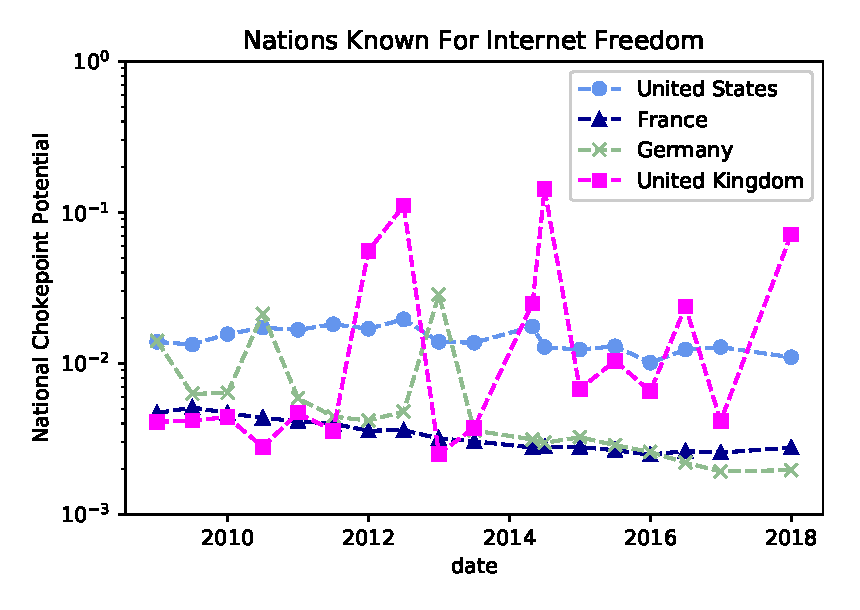
\includegraphics[width=\linewidth]{NodesFree}
	\caption{The number of border ASes required for the US, France, Germany, and Great Britain to intercept 90\% of in-to-out paths over time.}\label{fig:nodesFree}
\end{figure}
\begin{figure}
	\centering
	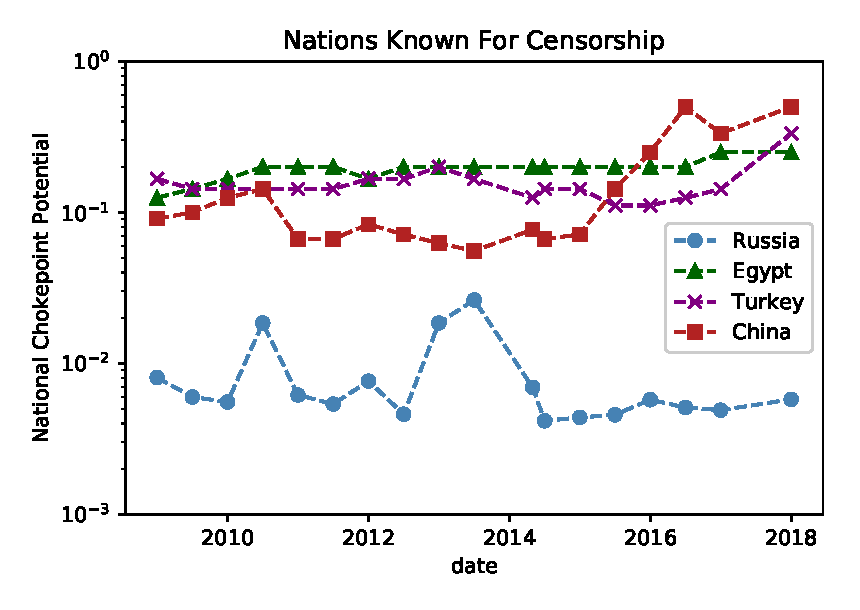
\includegraphics[width=\linewidth]{NodesCensor}
	\caption{The number of border ASes required for Russia, Egypt, Turkey, and China to intercept 90\% of in-to-out paths over time.}\label{fig:nodesCensor}
\end{figure}
\begin{figure*}
	\centering
	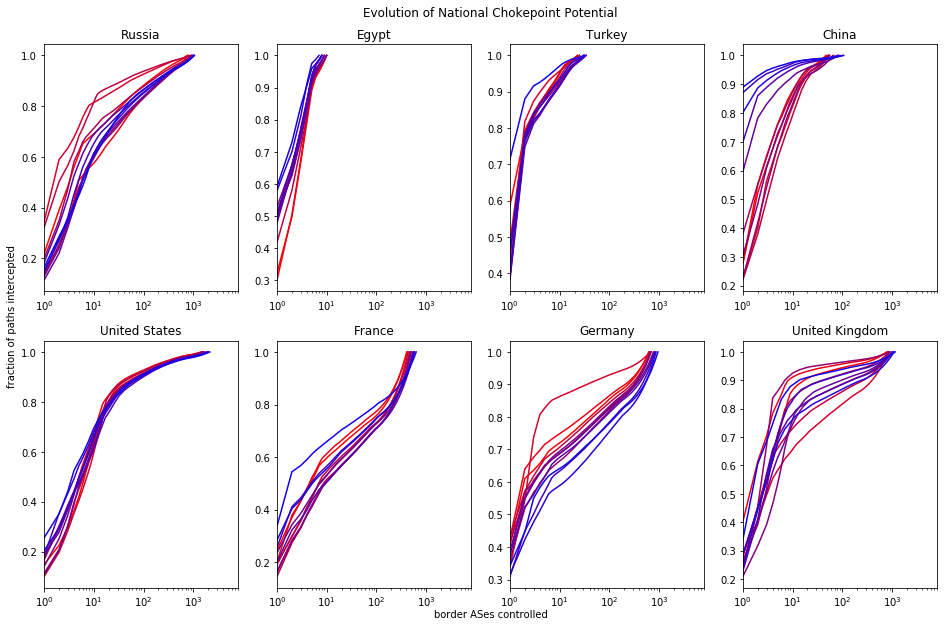
\includegraphics[width=\textwidth]{multi}
	\caption{Chokepoint potential (in-to-out) for multiple years
          \timerange. Each plot shows the number of border ASes
          controlled (x-axis) vs. $f$ (y-axis).}\label{fig:multiTime}
\end{figure*}

To study changes over time, we first plotted the
national chokepoint potential of each of the 8 selected countries
for each year (\figurename \ref{fig:nodesFree} and \figurename
\ref{fig:nodesCensor}).  The results are striking with a steep increase
over time for some nations (China and Turkey) and decreases for others
(Germany and France), while some countries remained relatively
stable. Given that the overall number of ASes and paths has increased
globally over time, it is likely that even nations that look stable
have in fact become more 'chokepointy' over time as some border ASes
must be intercepting more paths.  This fact makes the increased NCP observed
for some countries even more striking.

Next, for each country studied we sorted its border ASes so
that the first AS has the highest chokepoint potential.
%The sum of all these
%chokepoint potentials is 1.0.
Then, we calculated the cumulative chokepoint potential
%we step through the list, and record the
%cumulative chokepoint potential of all the ASes seen so far. If we
and plotted the
number of border ASes controlled vs cumulative chokepoint potential for each year in the study,
%This shows how many ASes are required to control a given
%percentage of paths.
as shown in
\figurename \ref{fig:multiTime}.  The x-axis (log-scale,
so countries with large differences can be compared more
easily) for each plot is the number of border ASes controlled, and the y-axis
is the fraction of in-to-out paths intercepted. Each line represents a different
year.
%, with the more red lines being farther in the past and more blue lines
%being more recent.

The U.S. and China exhibit dramatic differences. The U.S. has many
more ASes than China, so its line extends further to the right in the
plots. In all cases, China can control a much larger portion of its
paths with fewer ASes than the U.S., as expected. More interesting are
the trends over time.  China's topology has evolved such that very few
ASes can intercept nearly all BGP paths. For The U.S. it has become
somewhat easier to control most of its paths but more difficult to
intercept around 70\% of its paths and higher (yellow lines crossing
green lines).  This suggest an expansion of interior ASes with more
connections, as well as a strengthening of the very top ASes.
Not all nations have developed higher chokepoint potential, e.g., Germany shows a trend
in the opposite direction, which persists for any level of border ASes.

\subsection{Internet Freedom}

To test the correlation between Internet Freedom and NCP, we plotted
FOTN scores vs. the number of border ASes required to intercept 90\% of in-to-out
paths and computed the Ordinary
Least Squares (OLS) fits, finding that the relationship is
statistically significant (e.g., p-value $\leq$ 0.0001 for 2017). The
relationship held for other years, and 
Fig. \ref{fig:fotn} shows a representative result (2017).  The relationship also holds for Freedom of the Press scores compared to NCP (Fig. \ref{fig:fotp}), p-value $\leq$ 0.001.

\begin{figure}
	\centering
	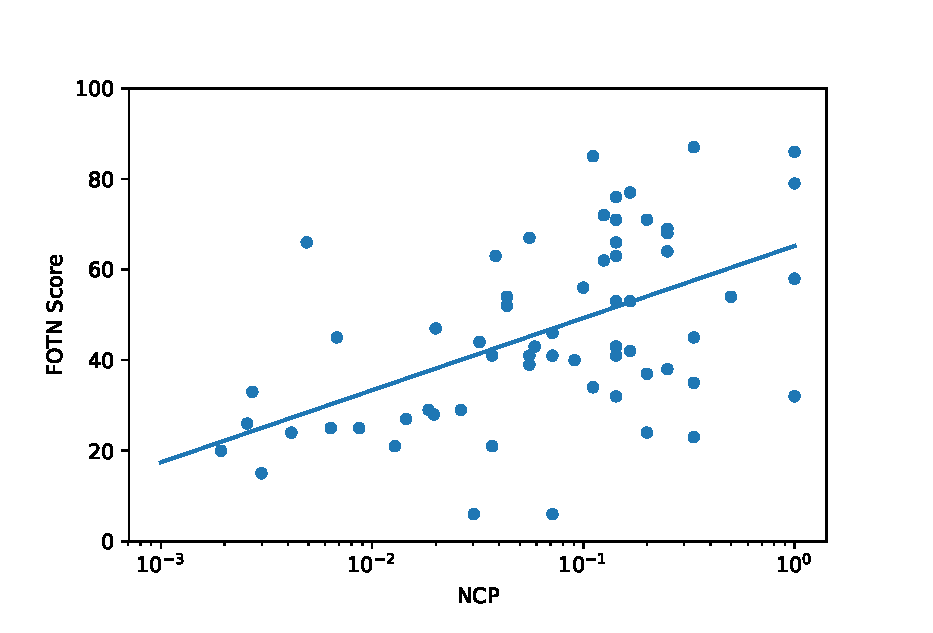
\includegraphics[width=\linewidth]{fotn}
	\caption{National Chokepoint Potential (in-to-out) vs. FOTN score
	for 2017. Higher FOTN scores indicate less freedom. The OLS fit is also plotted.}\label{fig:fotn}
\end{figure}

\begin{figure}
	\centering
	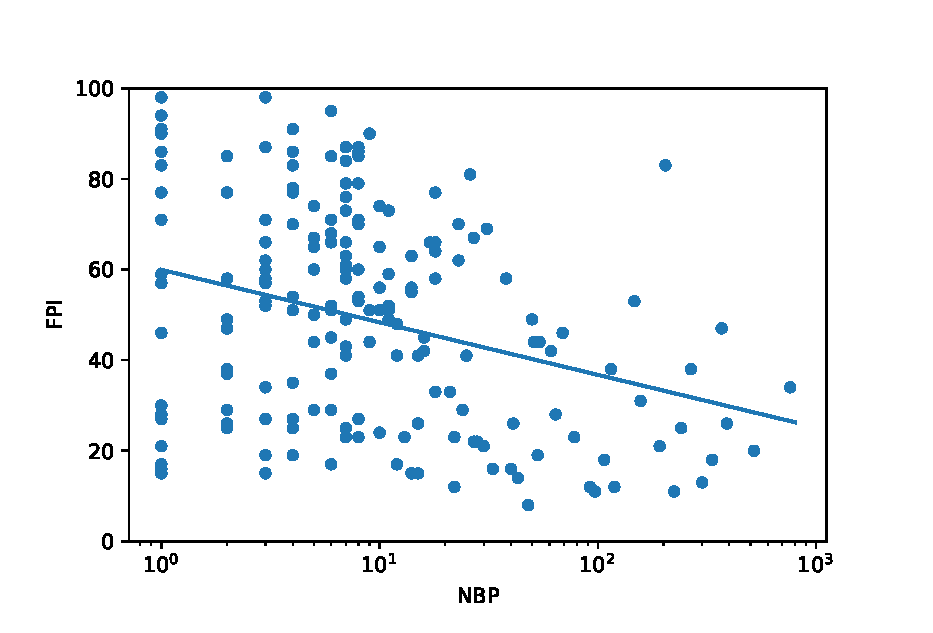
\includegraphics[width=\linewidth]{fotp}
	\caption{The National Chokepoint Potential (in-to-out) vs. FPI
	2017. Higher FPI indicates less freedom. The OLS fit is also plotted.}\label{fig:fotp}
\end{figure}

For each year there appear to be two general modes.  Nations that are
not free or partly free tend to have high NCP, while free nations have
variable NCPs. There are interesting outliers for both situations,
however. Countries like Estonia (EE) or Iceland (IS) are very free but
require few border ASes to control most of their paths. This is likely
because their overall AS counts are low. As we saw earlier, Russia
(RU) is considered not free by FOTN, but requires a large number of
ASes to control most of its paths. This suggests that censorship
in Russia is implemented without AS-level
chokepoints.
